\begin{frame}{Labeled Triangle}
\begin{center}
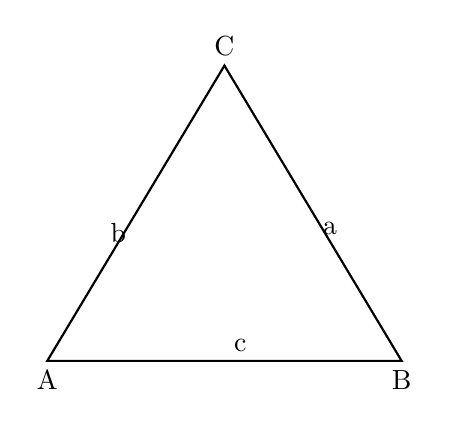
\begin{tikzpicture}[scale=1.5]
    \draw[thick] (0,0) -- (3,0) -- (1.5,2.5) -- cycle;
    \node[below] at (0,0) {A};
    \node[below] at (3,0) {B};
    \node[above] at (1.5,2.5) {C};
    \node[above right] at (1.5,0) {c};
    \node[below left] at (0.75,1.25) {b};
    \node[below right] at (2.25,1.25) {a};
\end{tikzpicture}
\end{center}

\footnotesize
\texttt{\textbackslash draw[thick] (0,0) -- (3,0) -- (1.5,2.5) -- cycle;}\\
\texttt{\textbackslash node[below] at (0,0) \{A\};}
\end{frame}